\section{Fourier Series}
\subsection{Motivation}

In the early 1800s, J. Fourier studied heat conduction along metal rot. This led him to investigate \(2 \pi\)-periodic functions, i.e., functions for which
\begin{equation}
    f\pqty{\theta + 2\pi} = f\pqty{\theta} \quad \forall \theta.
\end{equation}

Fourier made the following claim.

\begin{claim}[Fourier's Claim]
    Any \(2 \pi\)-periodic function can be expressed as a sum of complex exponentials in the form
    \begin{equation}
        f\pqty{\theta} = \sum_{n \in \ZZ} \hat{f}_n e^{i n \theta},
    \end{equation}
    and the coefficients \(\Bqty{\hat{f}_n}\) can be recovered as
    \begin{equation}
        \label{eq:fourier-claim-coefficient}%
        \hat{f}_n = \frac{1}{2\pi} \int_{0}^{2 \pi} f\pqty{\theta} e^{-i n \theta} \dd{\theta}.        
    \end{equation}
\end{claim}

This claim is not true in general, and we will discuss it in more details in a future section.

\subsection{Modern Treatment}

Consider the vector space
\begin{equation}
    V = \set{\functiondomain{f}{\RR}{\CC}}{
        f\pqty{\theta + L} = f\pqty{\theta} \quad \forall \theta \qand f \text{ is ``nice''}
    }.
\end{equation}

We note that it suffices for us to know the values over an interval of length \(L\), e.g., \(\cointv{0}{L}\), or \(\cointv{-\flatfrac{L}{2}}{\flatfrac{L}{2}}\). We equip \(V\) with an \term{inner product} \(\functiondomain{\inner   {\cdot}{\cdot}}{V \times V}{\CC}\) defined as
\begin{equation}
    \inner{f}{g} = \int_{0}^{L} f\pqty{\theta} \conjugate{g\pqty{\theta}} \dd{\theta}  = \int_{- \flatfrac{L}{2}}^{\flatfrac{L}{2}} f\pqty{\theta} \conjugate{g\pqty{\theta}} \dd{\theta}.
\end{equation}
associated with the norm
\begin{equation}
    \norm{f}^2 = \inner{f}{f} = \int_{0}^{L} f\pqty{\theta} \conjugate{f\pqty{\theta}} \dd{\theta}
\end{equation}

Consider the family of functions
\begin{equation}
    e_{n} \pqty{\theta} = \exp \pqty{\frac{2 \pi i n \theta}{L}}, \quad n \in \ZZ.
\end{equation}

Certainly, \(e_n \in V\) for all \(n \in \ZZ\), and the inner product satisfies
\begin{equation}
    \inner{e_m}{e_n} = \int_{0}^{L} \exp\pqty{\frac{2 \pi i m \theta}{L}} \exp\pqty{- \frac{2 \pi i n \theta}{L}} \dd{\theta} = \begin{cases}
        L, & m = n, \\
        0, & m \neq n,
    \end{cases}
\end{equation}
i.e., \(\inner{e_m}{e_n} = L \kronecker_{mn}\). So \(\Bqty{e_n}\) are orthogonal in \(V\) and \(\norm{e_n}^2 = L\).

Recall from \textit{IA Vectors and Matrices}, that if \(V_N\) is an \(N\)-dimensional vector space, and the set \(\Bqty{\vb{e}_n}_{n = 1}^{N}\) were orthogonal and \(\norm{\vb{e}_n}^2 = L\), then for any \(\vb{x} \in L_N\), we can write
\begin{equation}
    \vb{x} = \sum_{n = 1}^{N} \hat{x}_n \vb{e}_n,
\end{equation}
where we may extract the coefficients \(\hat{x}_n\) by a dot product:
\begin{subequations}
    \begin{align}
        \vb{x} \vdot \vb{e}_m &= \sum_{n = 1}^{N} \hat{x}_n \pqty{\vb{e}_n \vdot \vb{e}_m} \\
        &= \sum_{n = 1}^{N} \hat{x}_n L \kronecker_{nm} \\
        &= L \hat{x}_m.
    \end{align}
\end{subequations}

So for every \(\vb{x} \in V_N\), we have
\begin{equation}
    \vb{x} = \sum_{n = 1}^{N} \hat{x}_n \vb{e}_n, \quad \hat{x}_n = \frac{1}{L} \pqty{\vb{x} \vdot \vb{e}_n}.
\end{equation}

The question is can we do the same for \(V\), although \(V\) is not a finite-dimensional vector space (since no finite subset of \(\Bqty{e_n}_{n \in \ZZ}\) is linearly dependent)? Well, let's see what happens if we try to do the same.

Suppose an \(f \in V\) can be written in the form
\begin{equation}
    f\pqty{\theta} = \sum_{n \in \ZZ} \hat{f}_n e_n\pqty{\theta} = \sum_{n \in \ZZ} \hat{f}_n \exp\pqty{\frac{2 \pi i n \theta}{L}}.
\end{equation}

Then the coefficients can be identified similarly, by taking inner products, as
\begin{subequations}
    \begin{align}
        \inner{f}{e_m} &= \sum_{n \in \ZZ} \hat{f}_n \inner{e_n}{e_m} \\
        &= \sum_{n \in \ZZ} \hat{f}_n L \kronecker_{nm} \\
        &= L \hat{f}_m,
    \end{align}
\end{subequations}
which gives precisely
\begin{equation}
    \hat{f}_n = \frac{1}{L} \inner{f}{e_n} = \frac{1}{L} \int_{0}^{L} f\pqty{\theta} \exp\pqty{- \frac{2 \pi i n \theta}{L}} \dd{\theta}.
\end{equation}

Note that this is precisely the same as \autoref{eq:fourier-claim-coefficient} with \(L = 2 \pi\).

\begin{definition}
    For \(L\)-periodic function \(\functiondomain{f}{\RR}{\CC}\), we define its \term{complex Fourier coefficients} by the sum
    \begin{equation}
        \sum_{n \in \ZZ} \hat{f}_n \exp\pqty{\frac{2 \pi i n \theta}{L}}
    \end{equation}
    where the coefficients which satisfy
    \begin{equation}
        \hat{f}_n = \frac{1}{L} \int_{0}^{L} f\pqty{\theta} \exp\pqty{- \frac{2 \pi i n \theta}{L}} \dd{\theta}
    \end{equation}
    are called the \term{complex Fourier coefficients} of \(f\).

    Instead of writing an equal sign, we often use the symbol
    \begin{equation}
        f\pqty{\theta} \sim \sum_{n \in \ZZ} \hat{f}_n \exp\pqty{\frac{2 \pi i n \theta}{L}}
    \end{equation}
    which means that the right-hand side isthe Fourier series of the function on the left, \(f\).
\end{definition}

We would love to replace the sign ``\(\sim\)'' with simply an equal sign ``\(=\)'', but we cannot always do that.

We split this sum according to \(\Bqty{n = 0} \cup \Bqty{n > 0} \cup \Bqty{n < 0}\). Then we have
\begin{subequations}
    \begin{align}
        \sum_{n \in \ZZ} \hat{f}_n \exp\pqty{\frac{2 \pi i n \theta}{L}} &= \hat{f}_0 + \sum_{n = 1}^{\infty} \hat{f}_n \exp\pqty{\frac{2 \pi i n \theta}{L}} + \sum_{n = 1}^{\infty} \hat{f}_{-n} \exp\pqty{-\frac{2 \pi i n \theta}{L}} \\
        &= \hat{f}_0 + \sum_{n = 1}^{\infty} \hat{f_n} \bqty{\cos \pqty{\frac{2 \pi n \theta}{L}} + i \sin \pqty{\frac{2 \pi n \theta}{L}}} + \sum_{n = 1}^{\infty} \hat{f}_{-n} \bqty{\cos \pqty{\frac{2 \pi n \theta}{L}} - i \sin \pqty{\frac{2 \pi n \theta}{L}}} \\
        &= \hat{f}_0 + \sum_{n = 1}^{\infty} \bqty{\pqty{\hat{f}_n + \hat{f}_{-n}} \cos \pqty{\frac{2 \pi n \theta}{L}} + i \pqty{\hat{f}_n - \hat{f}_{-n}} \sin \pqty{\frac{2 \pi n \theta}{L}}}
    \end{align}
\end{subequations}

So we denote, for \(n \geq 0\), that
\begin{subequations}
    \begin{equation}
        a_n = \hat{f}_n + \hat{f}_{-n},
    \end{equation}
    \begin{equation}
        b_n = i \pqty{\hat{f}_n - \hat{f}_{-n}}.
    \end{equation}
\end{subequations}

\begin{definition}[Fourier Series]
    Given a \(L\)-periodic function \(\functiondomain{f}{\RR}{\CC}\), we define its \term{Fourier series} by the sum
    \begin{equation}
        \frac{1}{2} a_0 + \sum_{n = 1}^{\infty} \bqty{a_n \cos \pqty{\frac{2 \pi n \theta}{L}} + b_n \sin \pqty{\frac{2 \pi n \theta}{L}}}
    \end{equation}
    where the \term{Fourier coefficients} \(a_n\), \(b_n\) are defined by
    \begin{subequations}
        \begin{equation}
            a_n = \frac{2}{L} \int_{0}^{L} f\pqty{\theta} \cos \pqty{\frac{2 \pi n \theta}{L}} \dd{\theta}
        \end{equation}
        \begin{equation}
            b_n = \frac{2}{L} \int_{0}^{L} f\pqty{\theta} \sin \pqty{\frac{2 \pi n \theta}{L}} \dd{\theta}
        \end{equation}
    \end{subequations}
\end{definition}

Note that if \(f = f\pqty{\theta}\) is odd, then
\begin{subequations}
    \begin{align}
        a_n &= \frac{2}{L} \int_{0}^{L} f\pqty{\theta} \cos \pqty{\frac{2 \pi n \theta}{L}} \dd{\theta} \\
        &= \frac{2}{L} \int_{- \flatfrac{L}{2}}^{\flatfrac{L}{2}} f\pqty{\theta} \cos \pqty{\frac{2 \pi n \theta}{L}} \dd{\theta} \\
        &= 0,
    \end{align}
\end{subequations}
and similarly, if \(f\) is even,
\begin{subequations}
    \begin{align}
        b_n &= \frac{2}{L} \int_{0}^{L} f\pqty{\theta} \sin \pqty{\frac{2 \pi n \theta}{L}} \dd{\theta} \\
        &= \frac{2}{L} \int_{- \flatfrac{L}{2}}^{\flatfrac{L}{2}} f\pqty{\theta} \sin \pqty{\frac{2 \pi n \theta}{L}} \dd{\theta} \\
        &= 0.
    \end{align}
\end{subequations}

It is always a good idea to draw the graph of the function \(f\) before calculating its Fourier coefficients -- if the function is very nicely-behaved, then the Fourier coefficients should decay very quickly, and if the function is not so nicely-behaved, then the Fourier coefficients will decay more slowly.

\begin{figure}[ht!]
    \centering
    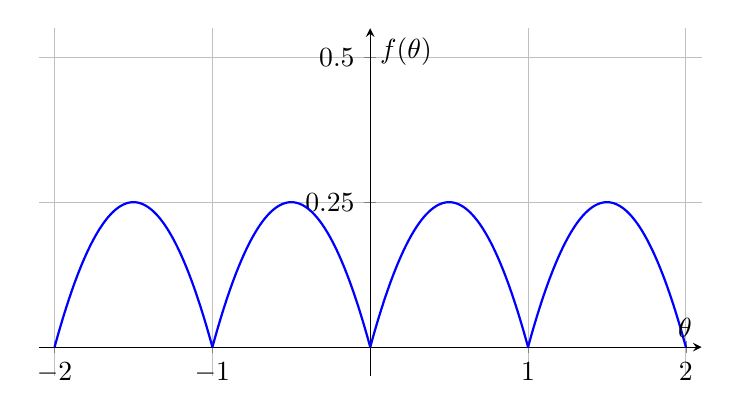
\begin{tikzpicture}
        \begin{axis}[
            axis lines = middle,
            xlabel = {$\theta$},
            ylabel = {$f(\theta)$},
            xmin = -2.1, xmax = 2.1,
            ymin = -0.05, ymax = 0.55,
            xtick = {-2,-1,0,1,2},
            ytick = {0, 0.25, 0.50},
            samples = 100,
            smooth,
            width = 10cm,
            height = 6cm,
            grid = both,
        ]
            \foreach \k in {-2,-1,0,1} {
                \addplot[thick, blue, domain=\k:\k+1]
                    {(x-\k)*(1-(x-\k))};
            }
        \end{axis}
    \end{tikzpicture}
    \caption{Function in \autoref{ex:fourier-series-example}}
    \label{fig:fourier-series-example}%
\end{figure}


\begin{example}
    \label{ex:fourier-series-example}%
    Define a \(1\)-periodic function \(\functiondomain{f}{\RR}{\RR}\) such that \(f\pqty{\theta} = \theta \pqty{1 - \theta}\) on \(\cointv{0}{1}\). Its graph is shown in \autoref{fig:fourier-series-example}.

    Through some computation, we find that \(\hat{f}_0 = \frac{1}{6}\). For \(n \neq 0\), through integration by parts,
    \begin{subequations}
        \begin{align}
            \hat{f}_n &= \int_{0}^{1} \theta \pqty{1 - \theta} e^{- 2 \pi i n \theta} \dd{\theta} \\
            &= - \frac{1}{2 \pi i n} \rightbar{\theta \pqty{1 - \theta} e^{- 2\pi i n \theta}}_{\theta = 0}^{1} + \frac{1}{2 \pi i n} \int_{0}^{1} \pqty{1 - 2 \theta} e^{- 2 \pi i n \theta} \dd{\theta} \\
            &= - \frac{1}{\pqty{2 \pi i n}^2} \rightbar{\pqty{1 - 2 \theta} e^{- 2 \pi i n \theta}}_{\theta = 0}^{1} \\
            &= - \frac{1}{2 \pqty{\pi n}^2}.
        \end{align}
    \end{subequations}
    noting that the first boundary terms vanish due to continuity. So
    \begin{equation}
        f\pqty{\theta} \sim \frac{1}{6} - \sum_{n \neq 0} \frac{1}{2 \pqty{\pi n}^2} e^{2 \pi i n \theta}
    \end{equation}
    or equivalently,
    \begin{equation}
        f\pqty{\theta} \sim \frac{1}{6} - \sum_{n = 1}^{\infty} \frac{1}{\pqty{\pi n}^2} \cos\pqty{2 \pi n \theta}.
    \end{equation}

    In this example, we indeed have an equality.
\end{example}